\section{Overview of neutron \el\ experiments}
\subsection{Neutron detection}
Neutron detection: fast plastic, liquid scintillators, He3 counter, CLYC array, poly
terphenyl. N-gamma discrimination by pulse shape discrimination. TOF techniques
for energy determination. Charged particle rejection. MoNA, neutron wall at
FRIB, VANDAL. Use of machine learning to distinguish gammas from neutrons.

Analog vs. digital techniques (connect to LANSCE measurements from \ref{Abfalterer2001, Finlay1993}).

\section{Sample Preparation}
\section{Experimental Facility at TUNL}
\section{Data Acquisition}

We conducted our neutron elastic cross section measurements at the neutron TOF
beamline of the Triangle Universities Nuclear Laboratory (TUNL) facility
(shown in Fig. \ref{ExperimentalSetupTUNL}).

\begin{figure}
  \begin{center}
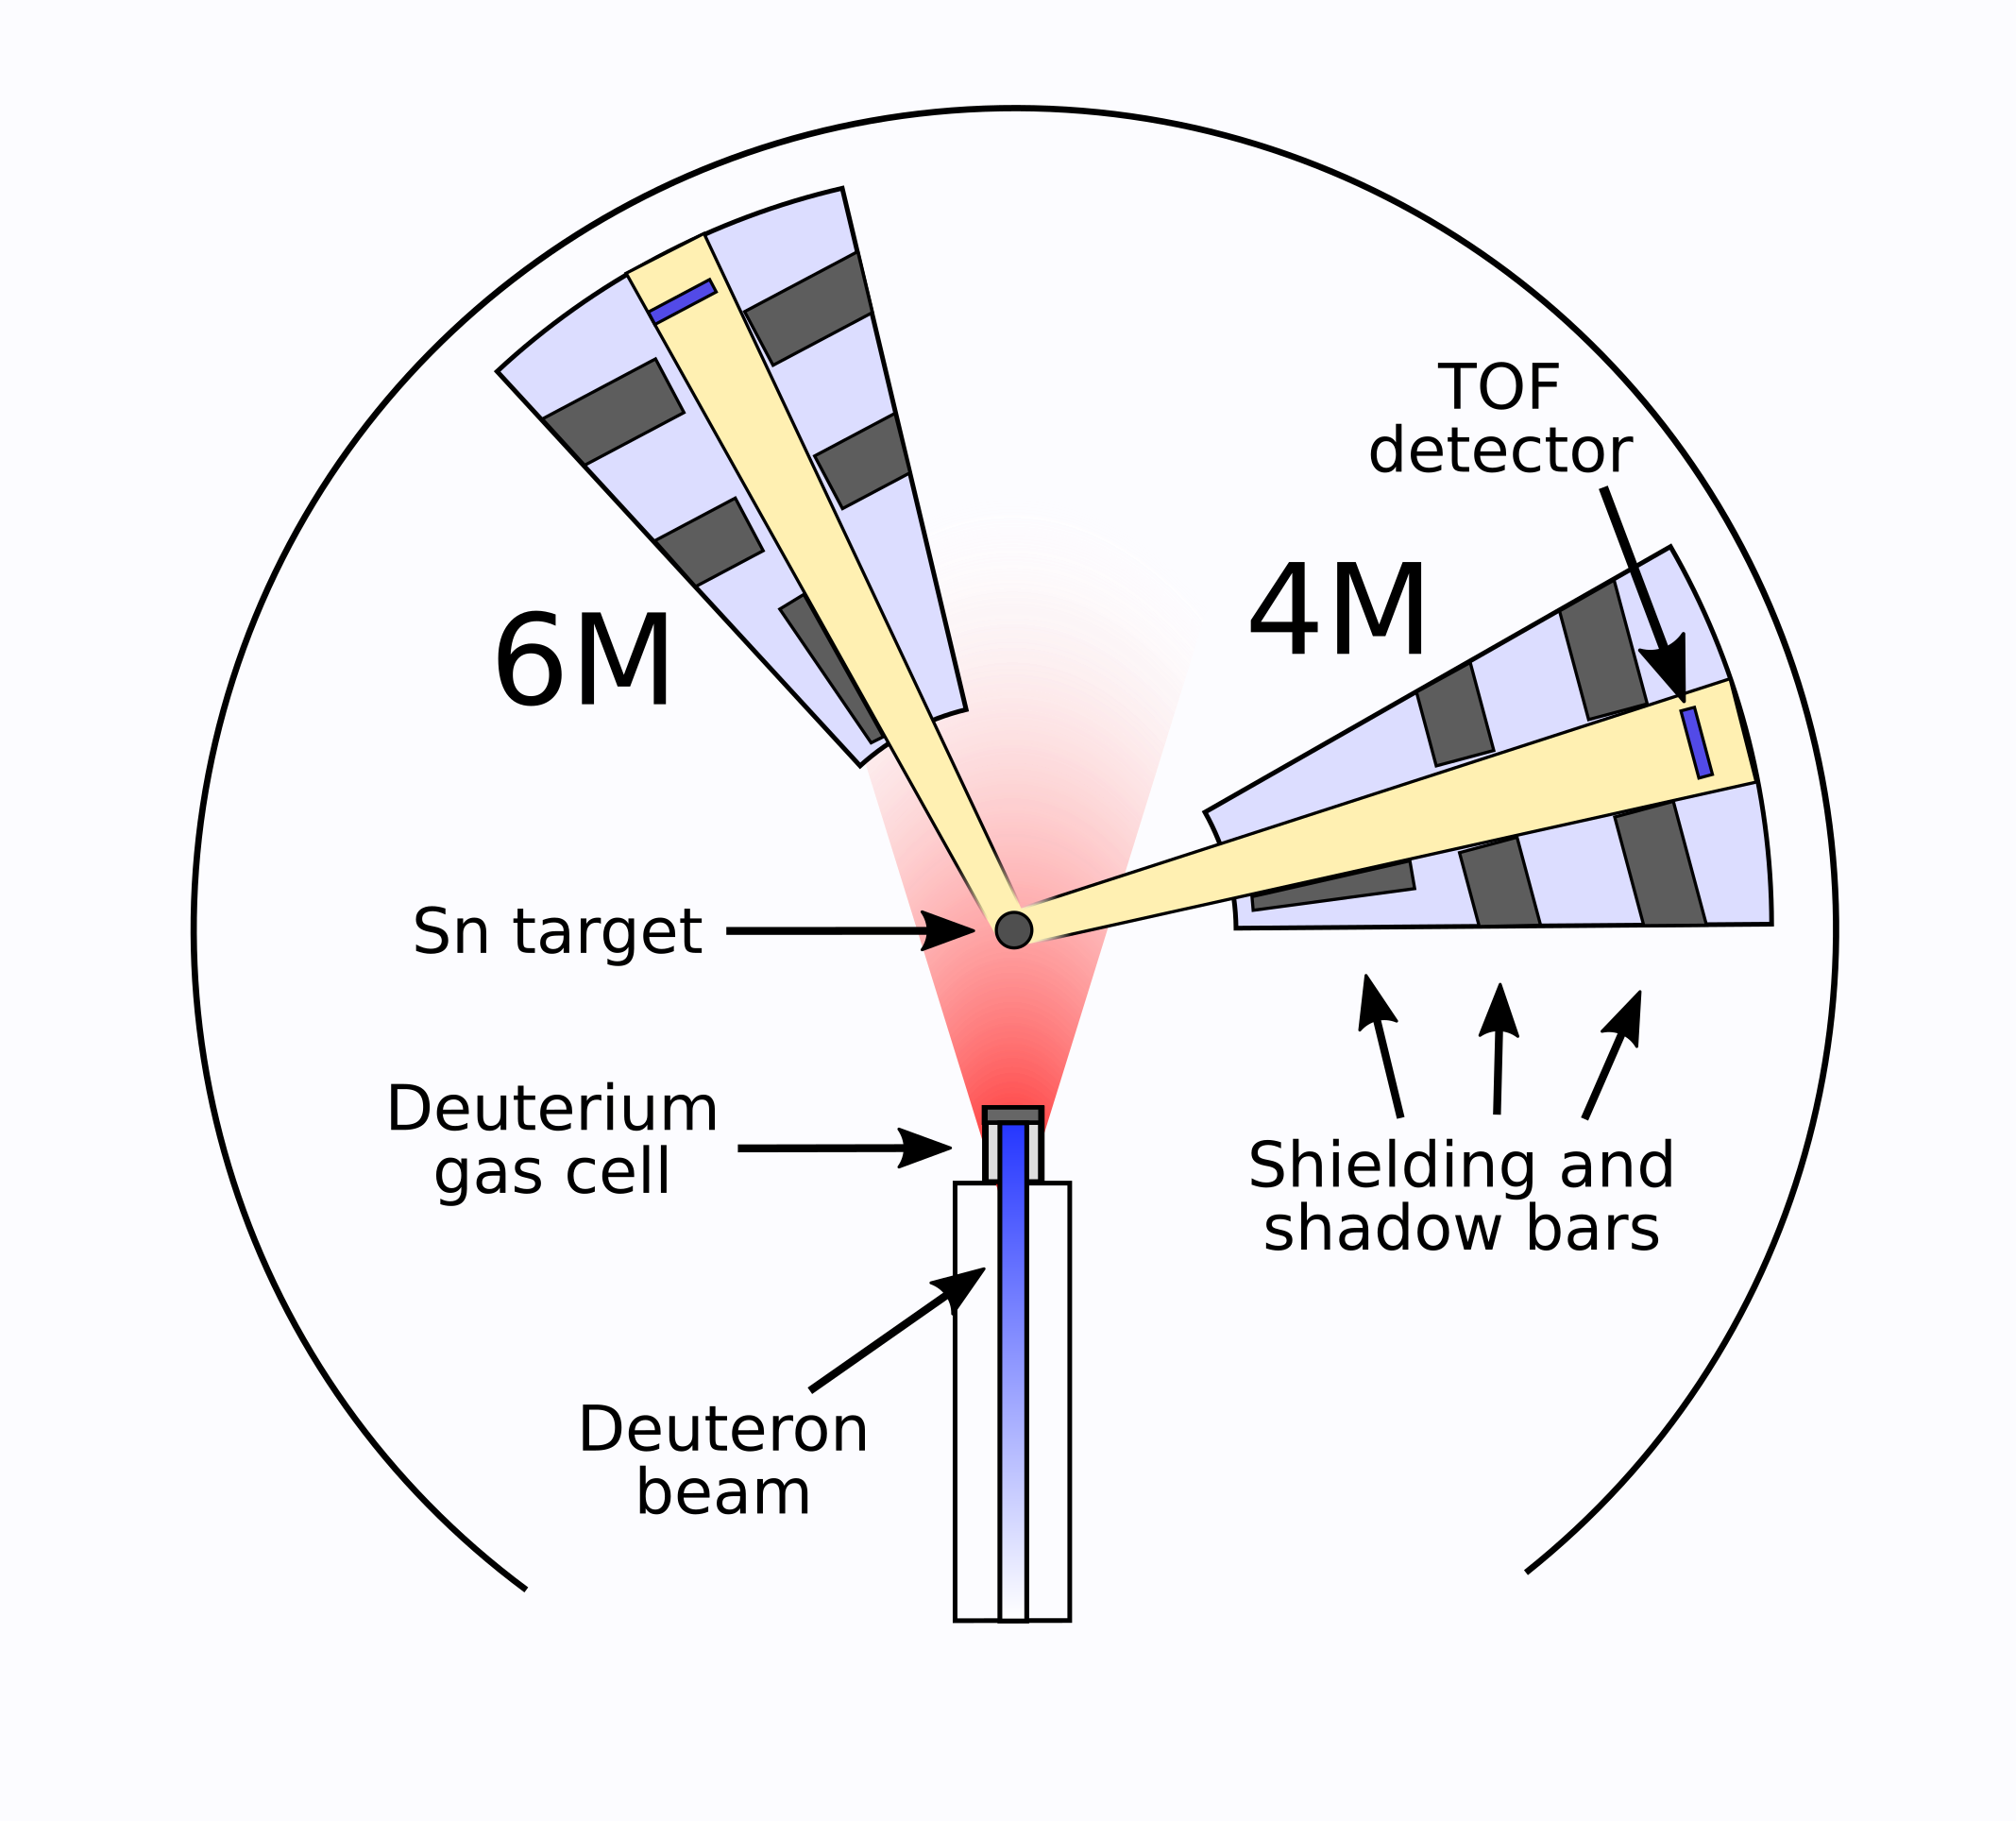
\includegraphics[width = 0.9\textwidth]{figures/ExperimentalSetupTUNL.png}
\caption{A diagram of the neutron TOF room at TUNL.} 
\label{ExperimentalSetupTUNL}
\end{center}
\end{figure}

\begin{figure}
  \begin{center}
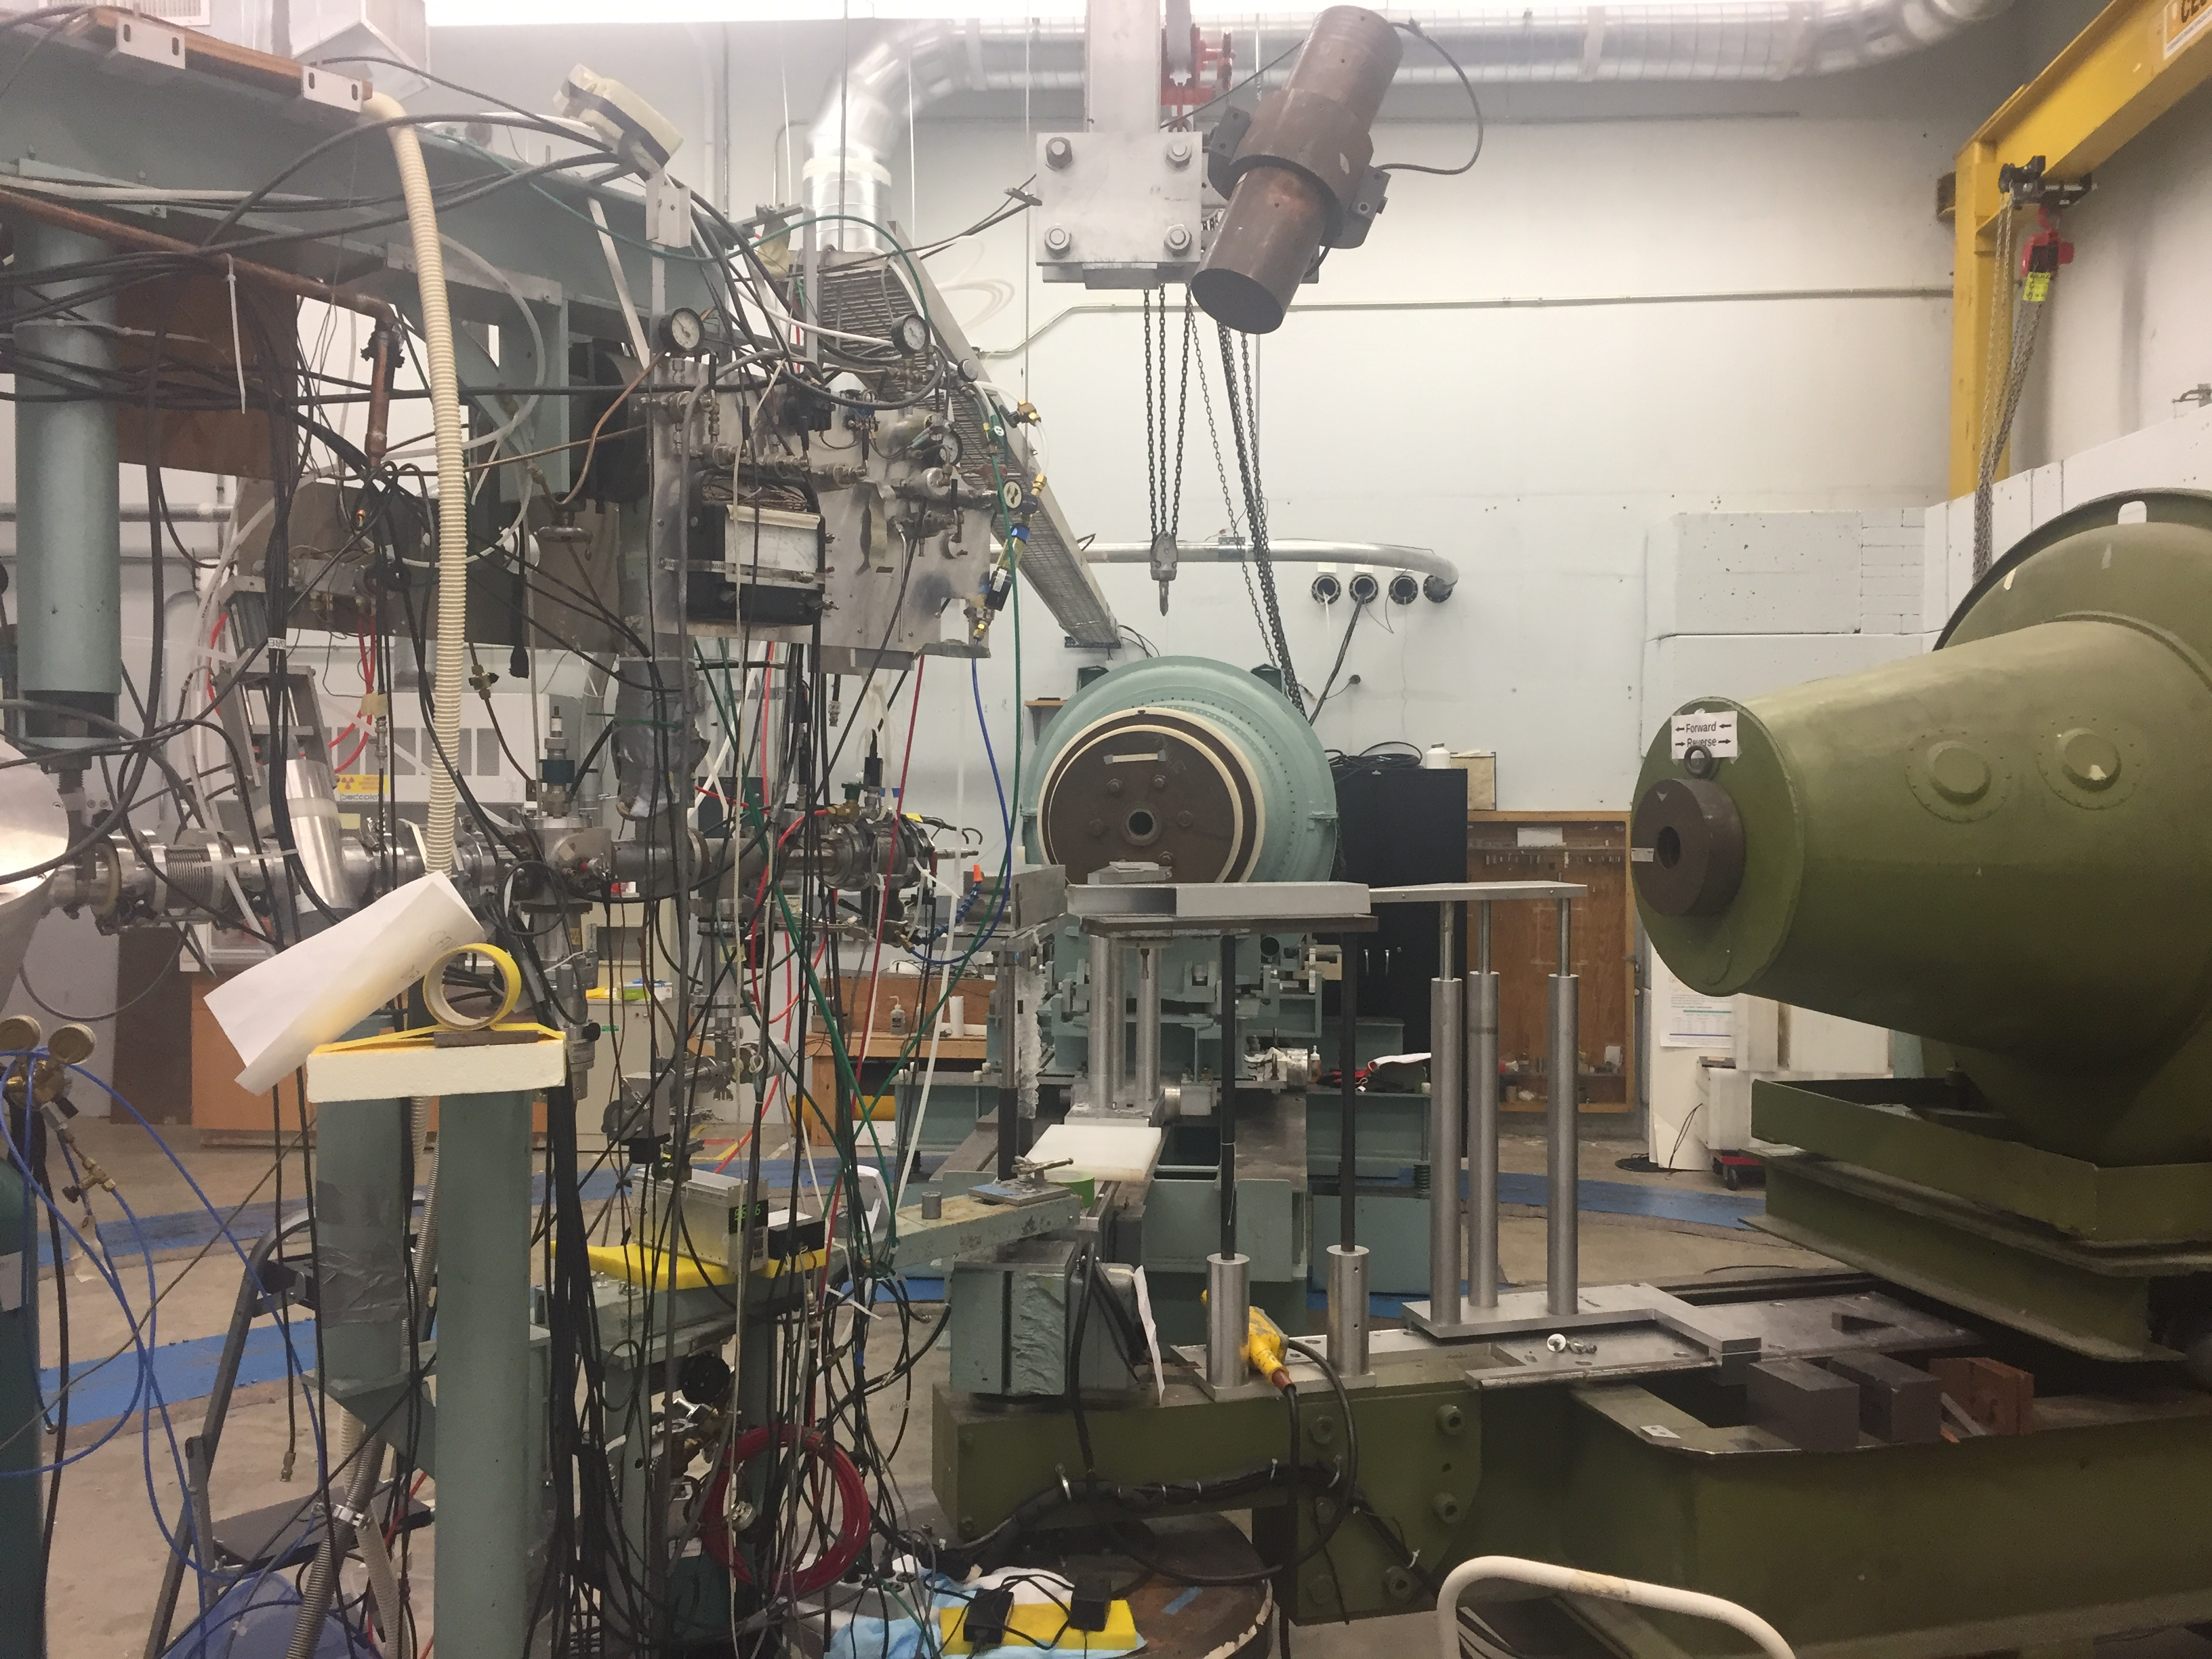
\includegraphics[width = 0.9\textwidth]{figures/TOFRoomPhoto.jpg}
\caption{Image of the neutron TOF room at TUNL.} 
\label{TOFRoomPhoto}
\end{center}
\end{figure}

Incident deuterons, supplied by the facility's variable-energy tandem
    Van De Graaf accelerator, impinged on a deuterium gas cell to produce a
forward-focused neutron beam via the d(d,n)3He reaction. Given the beam profile,
    the neutron energy distribution was calculated as X (Y) MeV with a FWHM of x (y)
    MeV for the 11 MeV and 17 MeV experiments, respectively. The gas cell was
    equipped with a tantalum beam stop to prevent unreacted beam from reaching
    the samples. 

    Samples were suspended in a vertically-aligned wire basket [INSERT DISTANCE] cm
    downstream of the gas cell and were rotated in and out of beam between
    runs with a hand-actuated pulley. Neutron scattering off
    the in-beam samples were recorded by one of the two main detectors, labeled ``4M"
    and ``6M". These detectors were mounted on large, movable carriages, or "arms",
    each of which was independently movable so that two angular cross section
    measurements could be conducted simultaneously. By recessing them deep within
    the arms' heavy shielding, the detectors were only accessible to neutrons
    entering the arm at a precise angle. The distance of the 4M (6M) angular
    detector from the sample was X (Y) cm, which, for an elastically-scattered
    11 MeV neutron, corresponds to a [insert time] ([insert time]) ns time-of-flight.

    To further reduce room background and prevent neutrons from entering the arms directly
    from the gas cell, an ensemble of "shadow bars" (wedge-shaped tungsten bricks)
    were used to adjust the aperture at the entrance to the arms. After an arm's
    angle was changed, the shadow bars were aligned by hand so that the
    detector buried deep within the arm had no line-of-sight to the gas cell or the
    shielding of the other arm, but its line-of-sight to the entire sample volume was
    maintained. Any configuration in which the arms were in opposition (i.e., the
    angle between the arms was 180+-20 degrees) would allow neutrons scattered
    from one arm direct access to the detector of the other arm, so these
    configurations were avoided.

    Signal timing and pulse shape data were collected from four [liquid scintillator]
    detectors: one in each of the angular arms, one in a ceiling monitor
    (CMON), and one at zero degrees with respect to the beam (ZDEG). In addition,
    an RF pulse from the accelerator was collected to serve as a time-of-flight
    (TOF) stop signal any time an event was recorded on one of the four neutron
    detectors. Detectors were calibrated with standard 137Cs and 22Na sources. For
    the 4M (6M) detector, a time resolution of X (Y) ns was established.
